\documentclass[a4paper,10pt]{article}
\usepackage{tikz}
\usepackage[utf8]{inputenc}
\usepackage{listings}
% Er zijn talloze parameters ...
\lstset{language=C++, showstringspaces=false, basicstyle=\small,
  numbers=left, numberstyle=\tiny, numberfirstline=false,
  stepnumber=1, tabsize=8, 
  commentstyle=\ttfamily, identifierstyle=\ttfamily,
  stringstyle=\itshape}
\usepackage{amsmath}

%opening
\title{ Hogebomen }
\author{ Lisette de Schipper (s1396250) en Micky Faas (s1407937) }
\date{}

\begin{document}

\maketitle

\begin{abstract}
Blablabla
\end{abstract}

\section{Inleiding}
AVL-bomen, splay-bomen en treaps zijn klassieke datastructuren die ingezet worden om een verzameling gegevens te faciliteren. Het zijn zelfbalancerende binaire zoekbomen die elk een vorm van ruimte en/of tijd-effici\"entie aanbieden. Er worden experimenten verricht om de prestatie van deze zelf-balancerende zoekbomen te vergelijken aan de hand van ophaaltijd van data, mate van herstructurering en het verwijderen van knopen. Ook wordt de prestatie van deze zoekbomen uitgezet tegen de ongebalanceerde tegenhanger, de binaire zoekboom.

\section{Werkwijze}
De vier bomen zijn conceptueel eenvoudig en relatief makkelijk te implementeren. Voor alle vier de bomen wordt dezelfde zoekmethode gebruikt. Deze is in het slechtste geval O($logn$).
\subsection{Implementatie binaire zoekboom}
TO DO
\subsection{Implementatie AVL-bomen}
Knopen van een AVL-boom hebben een \emph{balansfactor}, die altijd -1, 0 of 1 moet zijn. In deze implementatie is de balansfactor de hoogte van de rechtersubboom min de hoogte van de linkersubboom. Dit houdt dus in dat de hoogte van de linkersubboom van de wortel met maar 1 knoop kan verschillen van de hoogte van de rechtersubboom van de wortel. Het moment dat de balansfactor van een knoop minder dan -1 of meer dan 1 wordt, moet de boom geherstructureerd worden, om deze eigenschap te herstellen. \\

Om de balansfactor voor elke knoop te berekenen, houdt elke knoop zijn eigen hoogte bij. De balansfactor van een knoop wordt hersteld door rotaties. De richting en de hoeveelheid van de rotaties hangt af van de vorm van de betreffende (sub)boom. De volgende twee vormen en hun spiegelbeelden kunnen voorkomen bij het verwijderen of toevoegen van een knoop: \\

\begin{center}
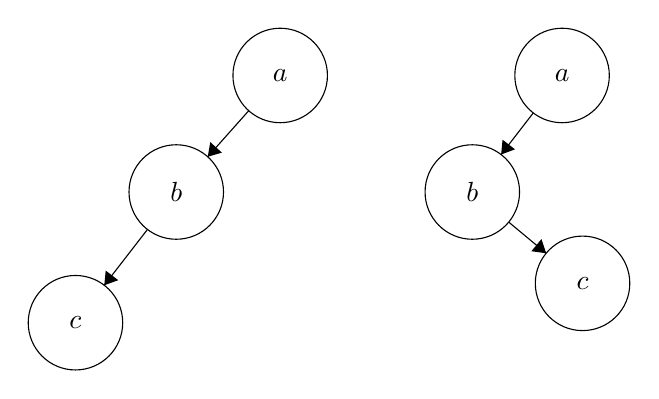
\begin{tikzpicture}[scale=0.2]
\tikzstyle{every node}+=[inner sep=0pt]
\draw [black] (16.5,-14.5) circle (3);
\draw (16.5,-14.5) node {$a$};
\draw [black] (9.9,-21.9) circle (3);
\draw (9.9,-21.9) node {$b$};
\draw [black] (34.4,-14.5) circle (3);
\draw (34.4,-14.5) node {$a$};
\draw [black] (3.5,-30.2) circle (3);
\draw (3.5,-30.2) node {$c$};
\draw [black] (28.7,-21.9) circle (3);
\draw (28.7,-21.9) node {$b$};
\draw [black] (35.7,-27.7) circle (3);
\draw (35.7,-27.7) node {$c$};
\draw [black] (14.5,-16.74) -- (11.9,-19.66);
\fill [black] (11.9,-19.66) -- (12.8,-19.4) -- (12.06,-18.73);
\draw [black] (32.57,-16.88) -- (30.53,-19.52);
\fill [black] (30.53,-19.52) -- (31.41,-19.19) -- (30.62,-18.58);
\draw [black] (31.01,-23.81) -- (33.39,-25.79);
\fill [black] (33.39,-25.79) -- (33.09,-24.89) -- (32.45,-25.66);
\draw [black] (8.07,-24.28) -- (5.33,-27.82);
\fill [black] (5.33,-27.82) -- (6.22,-27.5) -- (5.42,-26.89);
\end{tikzpicture}
\end{center}

In het eerste geval moet de wortel naar rechts worden geroteerd. In het tweede geval moeten we eerst naar de staat van de eerste subboom komen, door b naar links te roteren. Voor de spiegelbeelden van deze twee vormen geldt hetzelfde alleen in spiegelbeeld. \\

In deze implementatie van een AVL-boom bedraagt het toevoegen van een knoop in het ergste geval O($logn$) tijd, waarbij \emph{n} staat voor de hoogte van de boom. Eerst moet er gekeken worden of de data niet al in de boom voorkomt (O($logn$)) en vervolgens moet de boom op basis van de toevoeging geherstructureerd worden. Dit laatste is in het ergste geval O($logn$), omdat dan de gehele boom tot de wortel moeten worden nagelopen. \\

De complexiteitsgraad van het verwijderen van een knoop is gelijk aan die van het toevoegen van een knoop. In deze implementatie zoeken we in de rechtersubboom het kleinste kind en vervangen we de te verwijderen knoop met deze knoop. Dit heeft een duur van O($logn$). Als hij geen rechtersubboom heeft, wordt de node weggegooid en wordt zijn linkersubboom de nieuwe boom.
\subsection{Implementatie Splay-bomen}
TO DO
\subsection{Implementatie Treaps}
Treap lijkt in veel opzichten op een AVL-boom. De balansfactor per knoop heeft echter plaats gemaakt voor een prioriteit per knoop. Deze prioriteit wordt bij het toevoegen van een knoop willekeurig bepaald. De complexiteit voor het toevoegen en verwijderen van een knoop is hetzelfde als bij de AVL-boom. \\

Bij het toevoegen van een knoop moet er nog steeds omhoog gelopen worden in de boom, totdat de prioriteit van de toegevoegde knoop kleiner is dan de prioriteit van de ouder. Als dit niet het geval is, blijft de toegevoegde knoop omhoog roteren. In het ergste geval kan het dus weer zo zijn dat we tot de wortel door moeten blijven lopen. \\

Bij het verwijderen van een knoop blijven we de betreffende knoop roteren naar het kind met de grootste prioriteit. Uiteindelijk belanden we dan in de situatie dat de knoop maar een of geen kinderen heeft.
In het eerste geval verwijderen we de knoop en plakken zijn subboom terug aan de boom op zijn plek en in het tweede geval verwijderen we de knoop. In het slechtste geval duurt dit dus ook O($logn$) tijd.
\section{Onderzoek}

Een praktisch voorbeeld van binair zoeken in een grote boom is de spellingscontrole. Een spellingscontrole moet zeer snel voor een groot aantal strings kunnen bepalen of deze wel of niet tot de taal behoren. Aangezien er honderduizenden woorden in een taal zitten, is
lineair zoeken geen optie. Voor onze experimenten hebben wij dit als uitgangspunt genomen en hieronder zullen we kort de experimenten toelichten die wij hebben uitgevoerd. In het volgende hoofdstuk staan vervolgens de resultaten beschreven.

\subsection{Hooiberg}

``Hooiberg'' is de naam van het testprogramma dat we hebben geschreven speciaal ten behoeven van onze experimenten.
Het is een klein console programma dat woorden uit een bestand omzet tot een boom in het geheugen. 
Deze boom kan vervolgens worden doorzocht met de input uit een ander bestand: de ``naalden''.
De syntax is alsvolgt:
\begin{verbatim}
hooiberg type hooiberg.txt naalden.txt [treap-random-range]
\end{verbatim}
Hierbij is \texttt{type} \'e\'en van \texttt{bst, avl, splay, treap}, het eerste bestand bevat de invoer voor de boom, het tweede bestand een verzameling strings als zoekopdracht en de vierde parameters is voorbehouden voor het type \texttt{treap}.
De bestanden kunnen woorden of zinnen bevatten, gescheiden door regeleinden. De binaire bomen gebruiken lexicografische sortering 
die wordt geleverd door de operatoren \texttt{<} en \texttt{>} van de klasse \texttt{std::string}. Tijdens het zoeken wordt een
exacte match gebruikt (case-sensitive, non-locale-aware).

\subsection{Onderzoeks(deel)vragen}

Met onze experimenten hebben we gepoogd een aantal eenvoudige vragen te beantwoorden over het gebruik van de verschillende
binaire en zelf-organiserende bomen, te weten:

\begin{itemize}
\item Hoeveel meer rekenkracht kost het om grote datasets in te voegen in zelf-organiserende bomen tov binaire bomen?
\item Levert een zelf-organiserende boom betere zoekprestaties en onder welke opstandigheden?
\item Hoeveel extra geheugen kost een SOT?
\item Wat is de invloed van de random-factor bij de Treap?
\end{itemize}

\subsection{Meetmethoden}

Om de bovenstaande vragen te toetsen, hebben we een aantal meetmethoden bedacht.

\begin{itemize}
\item Rekenkracht hebben we gemeten in milliseconden tussen aanvang en termineren van een berekening. We hebben de delta's berekend rond de relevante code blokken dmv de C++11 \texttt{chrono} klassen in de Standard Template Library. Alle test zijn volledig sequentieel en single-threaded uitgevoerd. Deze resultaten zijn representatie voor \'e\'en bepaald systeem, vandaar dat we aantal \% `meer rekenkracht' als eenheid gebruiken.
\item Zoekprestatie hebben we zowel met rekenkracht als zoekdiepte gemeten. De zoekdiepte is het aantal stappen dat vanaf de wortel moet worden gemaakt om bij de gewenste knoop te komen. We hebben hierbij naar het totaal aantal stappen gekeken en naar de gemiddelde zoekdiepte.
\item Geheugen hebben we gemeten met de \texttt{valgrind} memory profiler. Dit programma wordt gebruikt voor het opsporen van geheugen lekken en houdt het aantal allocaties op de heap bij. Dit is representatie voor het aantal gealloceerde nodes. Aangezien hooiberg nauwelijks een eigen geheugen-voetafdruk heeft, zijn deze waarden representatief.
\end{itemize}

\subsection{Input data}

Voor ons experiment hebben we een taalbestand gebruikt van OpenTaal.org met meer dan 164.000 woorden. Dit is een relatief klein taalbestand, maar voldoede om verschillen te kunnen zien. We hebben een aantal testcondities gebruikt:
\begin{itemize}
\item Voor het inladen een wel of niet alfabetisch gesoorteerd taalbestand gebruiken.
\item Als zoekdocument hebben we een gedicht met 62 woorden gebruikt. Er zitten een aantal dubbele woorden in alsook een aantal woorden die niet in de woordenlijst voorkomen (werkwoordsvervoegingen).
\item We hebben ook een conditie waarbij we alle woorden gezocht hebben, zowel in dezelfde, als in een andere volgorde dan dat ze zijn ingevoerd.
\item We hebben \'e\'en conditie waarbij we de random-range van de Treap hebben gevari\"eerd.
\end{itemize}

\subsection{Hypothesen}

\begin{itemize}
\item De binairy search tree zal vermoedelijk het snelst nieuwe data toevoegen. De splay tree heeft veel ingewikkelde rotatie bij een insert, dus deze zal het traagst zijn.
\item Bij het gedicht zal de splay boom waarschijnlijk het snelst zijn omdat deze optimaliseert voor herhalingen.
\item ...
\item De bomen die een aparte node-klasse gebruiken (avl en treap) gebruiken het meeste geheugen.
\item De meest effici\"ente randomfactor is afhankelijk van de grootte van de boom die geïmplementeerd gaat worden. Bij een kleine boom volstaat een kleine randomfactor, bij een grote boom volstaat een grote randomfactor.
\end{itemize}

\section{Resultaten}

\section{Conclusies}

\section{Appendix}

\subsection{main.cc}
\lstinputlisting{../src/main.cc}
\subsection{hooiberg.cc}
\lstinputlisting{../src/hooiberg.cc}
\subsection{Tree.h}
\lstinputlisting{../src/Tree.h}
\subsection{TreeNode.h}
\lstinputlisting{../src/TreeNode.h}
\subsection{TreeNodeIterator.h}
\lstinputlisting{../src/TreeNodeIterator.h}
\subsection{SelfOrganizingTree.h}
\lstinputlisting{../src/SelfOrganizingTree.h}
\subsection{BinarySearchTree.h}
\lstinputlisting{../src/BinarySearchTree.h}
\subsection{BSTNode.h}
\lstinputlisting{../src/BSTNode.h}
\subsection{AVLTree.h}
\lstinputlisting{../src/AVLTree.h}
\subsection{AVLNode.h}
\lstinputlisting{../src/AVLNode.h}
\subsection{SplayTree.h}
\lstinputlisting{../src/SplayTree.h}
\subsection{Treap.h}
\lstinputlisting{../src/Treap.h}
\subsection{TreapNode.h}
\lstinputlisting{../src/TreapNode.h}
\end{document}
